%*************************************************************************
\section{Integration eigener Matching-Engines} \label{sec:own_matching_engine}
%*************************************************************************

Wie bereits erwähnt lassen sich auch eigene Matching-Engines in die SiLift-Processing-Pipeline integrieren.\\
Erstellen Sie dazu über \texttt{File} $\triangleright$ \texttt{New} $\triangleright$ \texttt{Other...}: \texttt{Plug-in Development} $\triangleright$ \texttt{Plug-in Project} eines neues Plugin und öffnen Sie die \texttt{MANIFEST.MF}.
Wechseln Sie auf den Reiter \texttt{Dependencies} und fügen Sie die in Abbildung \ref{silift-plugin_matcher_manifest_dependencies} markierten Abhängigkeiten hinzu.

\begin{figure}[H]
\centering
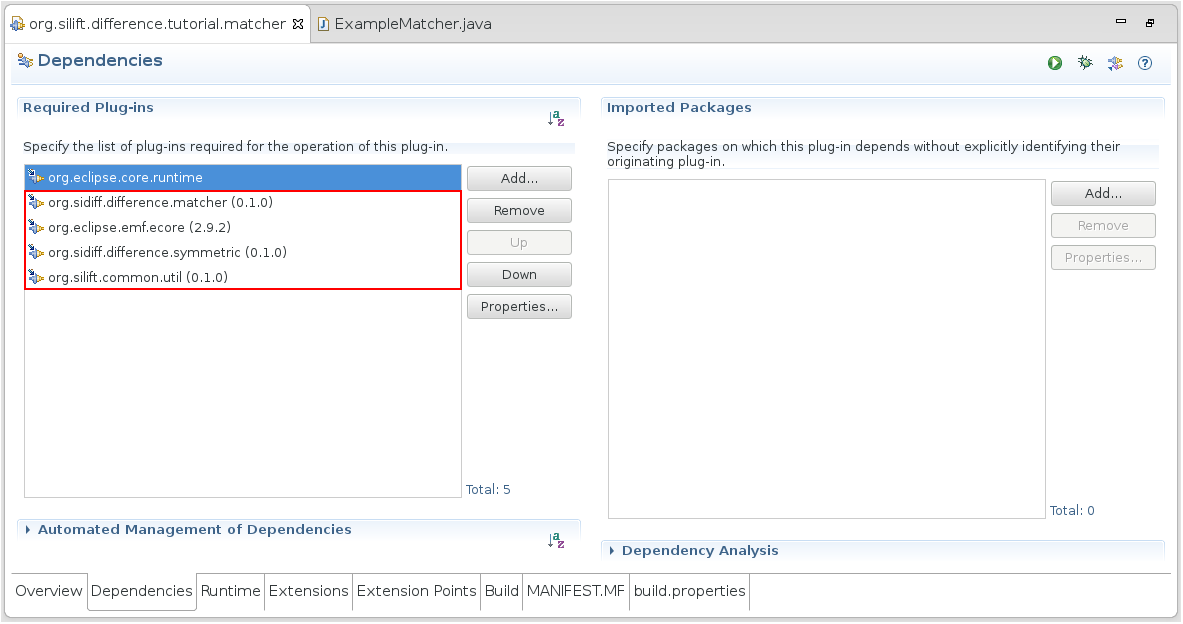
\includegraphics[width=0.8\textwidth]{matching/graphics/silift-plugin_matcher_manifest_dependencies}
\caption{\texttt{MANIFEST.MF} $\triangleright$ \texttt{Dependencies}}
\label{silift-plugin_matcher_manifest_dependencies}
\end{figure}

Als nächstes wird eine Klasse benötigt die die Schnittstelle \texttt{IMatcher} implementiert (vgl. Abb. \ref{silift-plugin_matcher_imatcher}).
Neben den zu implementierenden Methoden ist es Ihnen frei gestellt, ob sie Ihren Matcher in dieser Klasse implementieren oder diese nur als Adapter für einen ausgelagerten Matcher nutzen.

\begin{figure}[H]
\centering
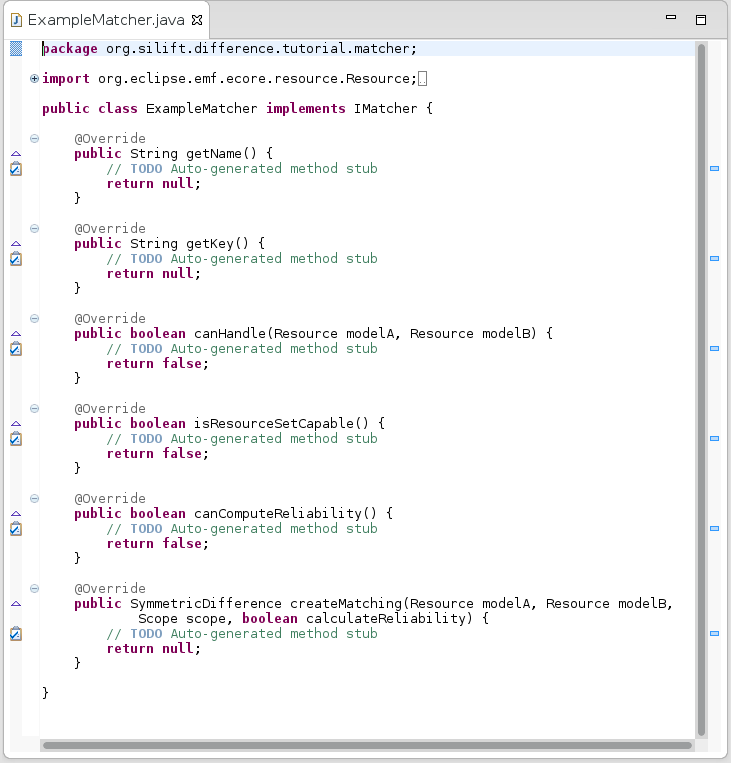
\includegraphics[width=0.6\textwidth]{matching/graphics/silift-plugin_matcher_imatcher.png}
\caption{Klasse \texttt{ExampleMatcher} implementiert \texttt{IMatcher}}
\label{silift-plugin_matcher_imatcher}
\end{figure}

Anstatt die Schnittstelle \texttt{IMatcher} von Grund auf zu implementieren, kann auch die ``Convenience''-Klasse \texttt{BaseMatcher} erweitert werden (vgl. Abb. \ref{silift-plugin_matcher_basematcher}).
Diese stellt bereits Methoden zum Iterieren über die Modellelemente bereit.
Zusätzlich muss noch die Methode \texttt{isCorresponding} implementiert werden.

\begin{figure}[H]
\centering
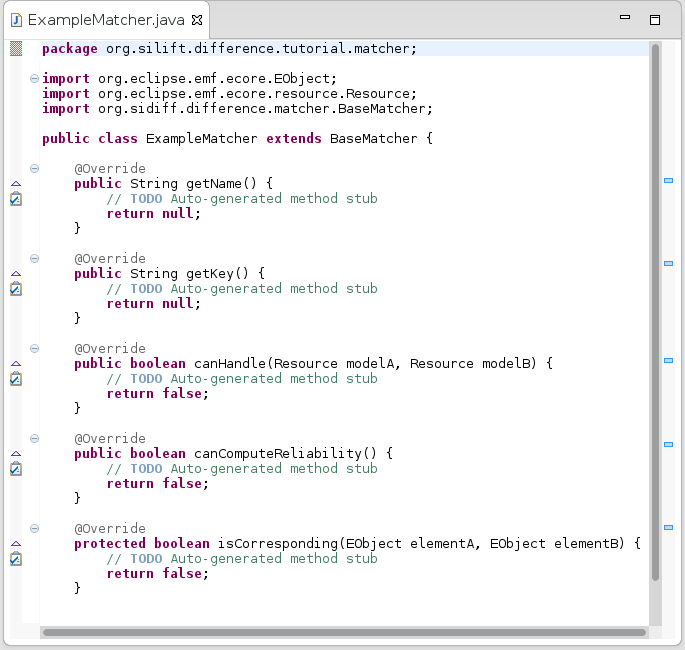
\includegraphics[width=0.6\textwidth]{matching/graphics/silift-plugin_matcher_basematcher.png}
\caption{Klasse \texttt{ExampleMatcher} erweitert \texttt{BaseMatcher}}
\label{silift-plugin_matcher_basematcher}
\end{figure}

Danach muss das Plugin noch als Extension für \texttt{SiLift} definiert werden.
Gehen Sie dazu wieder in die \texttt{MANIFEST.MF} und wechseln Sie auf den Reiter \texttt{Extensions} (vgl. Abb. \ref{silift-plugin_matcher_manifest_extensions}).

\begin{figure}[H]
\centering
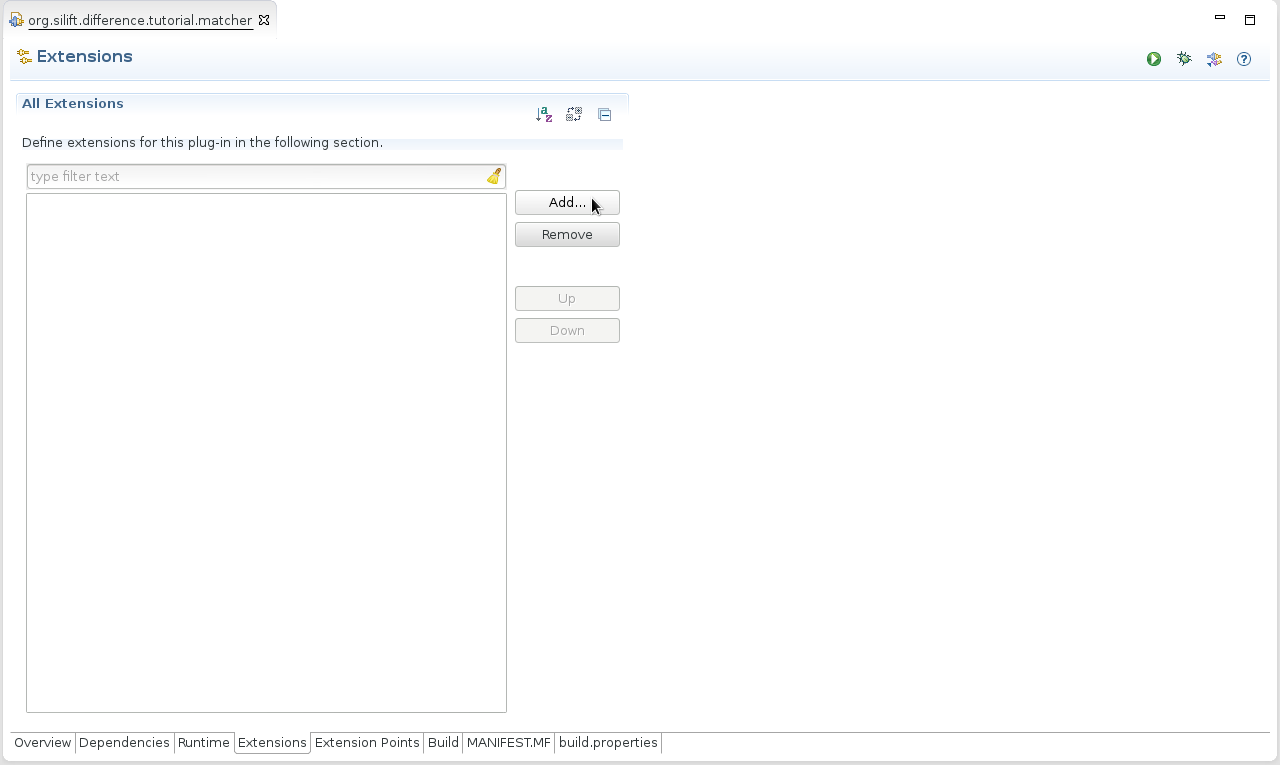
\includegraphics[width=0.8\textwidth]{matching/graphics/silift-plugin_matcher_manifest_extensions.png}
\caption{\texttt{MANIFEST.MF} $\triangleright$ \texttt{Extensions}}
\label{silift-plugin_matcher_manifest_extensions}
\end{figure}

Klicken Sie auf auf \texttt{Add...} und selektieren Sie den \textit{Extension Point} \texttt{org.""sidiff.""difference.""matcher.""matcher\_""extension} (vgl. Abb. \ref{silift-plugin_matcher_manifest_add_extension_point}).

\begin{figure}[H]
\centering
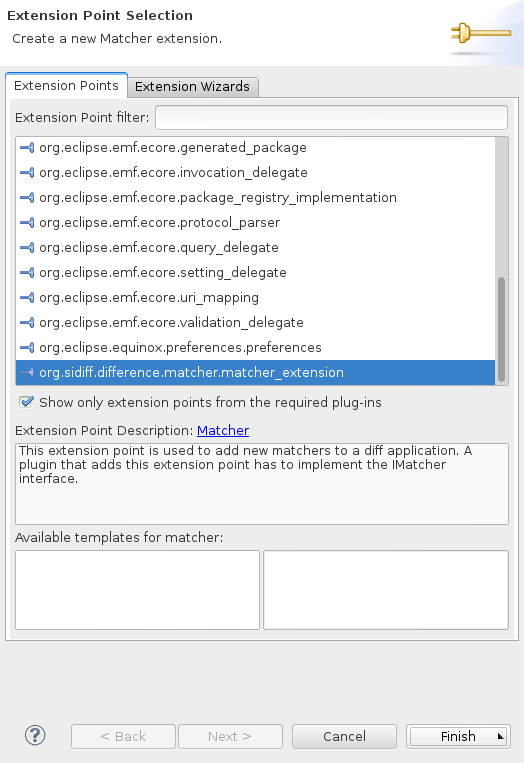
\includegraphics[width=0.6\textwidth]{matching/graphics/silift-plugin_matcher_manifest_add_extension_point.png}
\caption{\texttt{MANIFEST.MF} $\triangleright$ \texttt{Extensions}: Extension Point Selection}
\label{silift-plugin_matcher_manifest_add_extension_point}
\end{figure}

Wechseln Sie in den Reiter \texttt{plugin.xml} und fügen dem eben erstellen Extension Point die entsprechende URI der Erweiterung bei (vgl. Abb. \ref{silift-plugin_matcher_manifest_plugin}).

\begin{figure}[H]
\centering
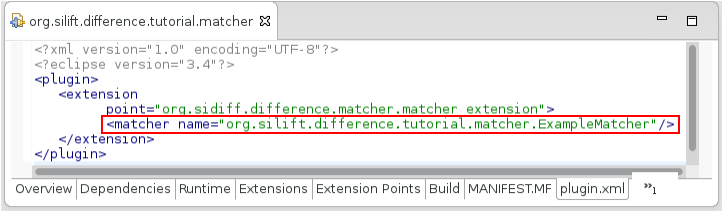
\includegraphics[width=0.6\textwidth]{matching/graphics/silift-plugin_matcher_manifest_plugin.png}
\caption{\texttt{MANIFEST.MF} $\triangleright$ \texttt{plugin.xml}}
\label{silift-plugin_matcher_manifest_plugin}
\end{figure}

Als letztes muss das Plugin noch \textit{deployed} werden.
Öffnen Sie mit der rechten Maustaste auf Ihrem Plugin-Projekt im Package Exploerer das Kontextmenü und klicken Sie auf \texttt{Export...} (vgl. Abb. \ref{silift-plugin_contextmenu_export}).

\begin{figure}[H]
\centering
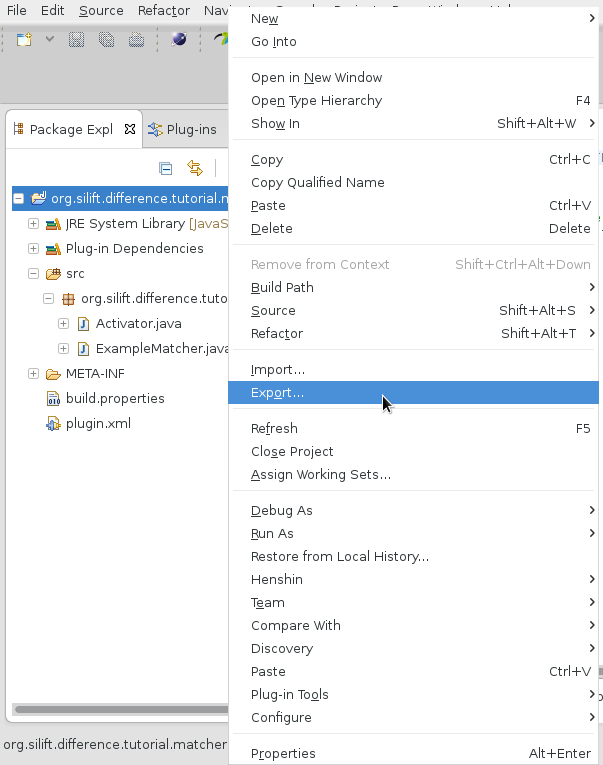
\includegraphics[width=0.6\textwidth]{matching/graphics/silift-plugin_contextmenu_export.png}
\caption{\texttt{Export Plugin}}
\label{silift-plugin_contextmenu_export}
\end{figure}

Selektieren Sie \texttt{Plug-in Development} $\triangleright$ \texttt{Deployable plug-ins and fragements} und klicken Sie \texttt{Next} (vgl. Abb. \ref{silift-plugin_wizard_deploy01}).

\begin{figure}[H]
\centering
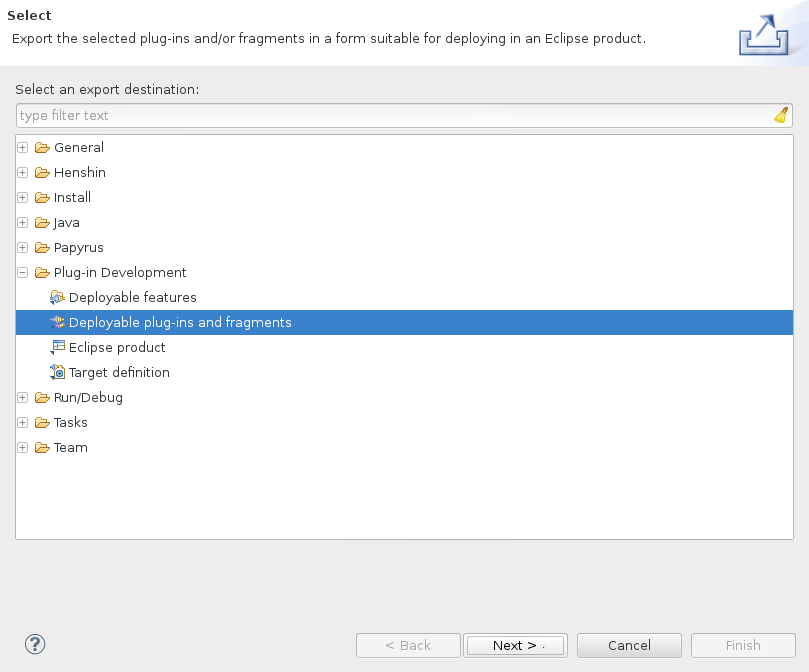
\includegraphics[width=0.6\textwidth]{matching/graphics/silift-plugin_wizard_deploy01.png}
\caption{\texttt{Export Wizard}: Page 1}
\label{silift-plugin_wizard_deploy01}
\end{figure}

Wählen Sie als nächstes \texttt{install into host.Repository} aus und geben Sie den Pfad zum Plugin-Ordner Ihrer Eclipse-Installation an (vgl. Abb. \ref{silift-plugin_wizard_deploy02}).
Klicken Sie auf \texttt{Finish} und starten Sie nach erfolgreicher Installation Ihr Eclipse neu.

\begin{figure}[H]
\centering
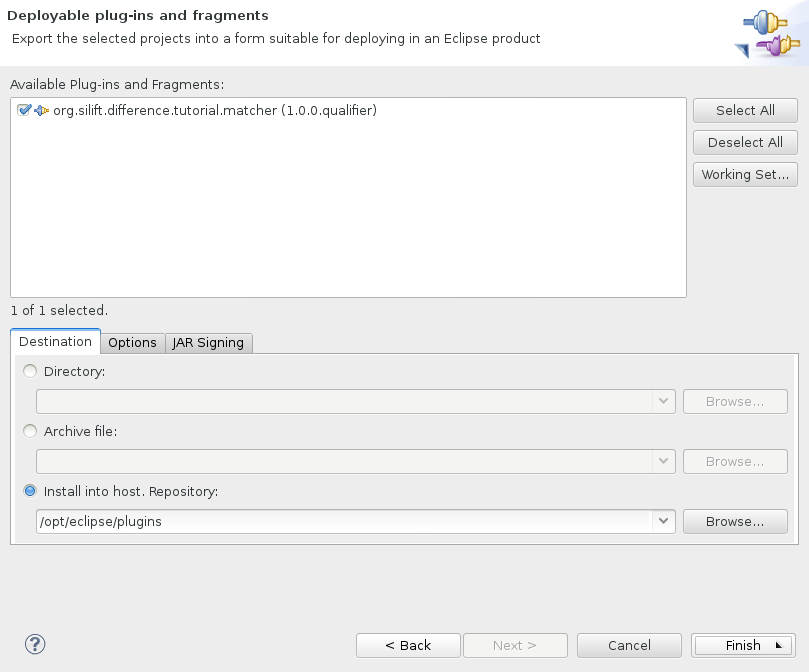
\includegraphics[width=0.6\textwidth]{matching/graphics/silift-plugin_wizard_deploy02.png}
\caption{\texttt{Export Wizard}: Page 2}
\label{silift-plugin_wizard_deploy02}
\end{figure}

Ihr Matcher kann nun in Verbindung mit SiLift genutzt werden.
